\chapter{Dynamic programming}

\index{dynamic programming}

\key{Dynamic programming}
is a technique that combines the correctness
of complete search and the efficiency
of greedy algorithms.
Dynamic programming can be applied if the
problem can be divided into overlapping subproblems
that can be solved independently.

There are two uses for dynamic programming:

\begin{itemize}
\item
\key{Finding an optimal solution}:
We want to find a solution that is
as large as possible or as small as possible.
\item
\key{Counting the number of solutions}:
We want to calculate the total number of
possible solutions.
\end{itemize}

We will first see how dynamic programming can
be used to find an optimal solution,
and then we will use the same idea for
counting the solutions.

Understanding dynamic programming is a milestone
in every competitive programmer's career.
While the basic idea is simple,
the challenge is how to apply
dynamic programming to different problems.
This chapter introduces a set of classic problems
that are a good starting point.

\section{Coin problem}

We first focus on a problem that we
have already seen in Chapter 6:
Given a set of coin values $\texttt{coins} = \{c_1,c_2,\ldots,c_k\}$
and a target sum of money $n$, our task is to
form the sum $n$ using as few coins as possible.

In Chapter 6, we solved the problem using a
greedy algorithm that always chooses the largest
possible coin.
The greedy algorithm works, for example,
when the coins are the euro coins,
but in the general case the greedy algorithm
does not necessarily produce an optimal solution.

Now is time to solve the problem efficiently
using dynamic programming, so that the algorithm
works for any coin set.
The dynamic programming
algorithm is based on a recursive function
that goes through all possibilities how to
form the sum, like a brute force algorithm.
However, the dynamic programming
algorithm is efficient because
it uses \emph{memoization} and
calculates the answer to each subproblem only once.

\subsubsection{Recursive formulation}

The idea in dynamic programming is to
formulate the problem recursively so
that the solution to the problem can be
calculated from solutions to smaller
subproblems.
In the coin problem, a natural recursive
problem is as follows:
what is the smallest number of coins
required to form a sum $x$?

Let $\texttt{solve}(x)$
denote the minimum
number of coins required for a sum $x$.
The values of the function depend on the
values of the coins.
For example, if $\texttt{coins} = \{1,3,4\}$,
the first values of the function are as follows:

\[
\begin{array}{lcl}
\texttt{solve}(0) & = & 0 \\
\texttt{solve}(1) & = & 1 \\
\texttt{solve}(2) & = & 2 \\
\texttt{solve}(3) & = & 1 \\
\texttt{solve}(4) & = & 1 \\
\texttt{solve}(5) & = & 2 \\
\texttt{solve}(6) & = & 2 \\
\texttt{solve}(7) & = & 2 \\
\texttt{solve}(8) & = & 2 \\
\texttt{solve}(9) & = & 3 \\
\texttt{solve}(10) & = & 3 \\
\end{array}
\]

For example, $\texttt{solve}(10)=3$,
because at least 3 coins are needed
to form the sum 10.
The optimal solution is $3+3+4=10$.

The essential property of $\texttt{solve}$ is
that its values can be
recursively calculated from its smaller values.
The idea is to focus on the \emph{first}
coin that we choose for the sum.
For example, in the above scenario,
the first coin can be either 1, 3 or 4.
If we first choose coin 1,
the remaining task is to form the sum 9
using the minimum number of coins,
which is a subproblem of the original problem.
Of course, the same applies to coins 3 and 4.
Thus, we can use the following recursive formula
to calculate the minimum number of coins:
\begin{equation*}
\begin{split}
\texttt{solve}(x) = \min( & \texttt{solve}(x-1)+1, \\
                           & \texttt{solve}(x-3)+1, \\
                           & \texttt{solve}(x-4)+1).
\end{split}
\end{equation*}
The base case of the recursion is $\texttt{solve}(0)=0$,
because no coins are needed to form an empty sum.
For example,
\[ \texttt{solve}(10) = \texttt{solve}(7)+1 = \texttt{solve}(4)+2 = \texttt{solve}(0)+3 = 3.\]

Now we are ready to give a general recursive function
that calculates the minimum number of
coins needed to form a sum $x$:
\begin{equation*}
    \texttt{solve}(x) = \begin{cases}
               \infty               & x < 0\\
               0               & x = 0\\
               \min_{c \in \texttt{coins}} \texttt{solve}(x-c)+1 & x > 0 \\
           \end{cases}
\end{equation*}

First, if $x<0$, the value is $\infty$,
because it is impossible to form a negative
sum of money.
Then, if $x=0$, the value is $0$,
because no coins are needed to form an empty sum.
Finally, if $x>0$, the variable $c$ goes through
all possibilities how to choose the first coin
of the sum.

Once a recursive function that solves the problem
has been found,
we can directly implement a solution in C++
(the constant \texttt{INF} denotes infinity):

\begin{lstlisting}
int solve(int x) {
    if (x < 0) return INF;
    if (x == 0) return 0;
    int best = INF;
    for (auto c : coins) {
        best = min(best, solve(x-c)+1);
    }
    return best;
}
\end{lstlisting}

Still, this function is not efficient,
because there may be an exponential number of ways
to construct the sum.
However, next we will see how to make the
function efficient using a technique called memoization.

\subsubsection{Using memoization}

\index{memoization}

The idea of dynamic programming is to use
\key{memoization} to efficiently calculate
values of a recursive function.
This means that the values of the function
are stored in an array after calculating them.
For each parameter, the value of the function
is calculated recursively only once, and after this,
the value can be directly retrieved from the array.

In this problem, we use arrays
\begin{lstlisting}
bool ready[N];
int value[N];
\end{lstlisting}

where $\texttt{ready}[x]$ indicates
whether the value of $\texttt{solve}(x)$ has been calculated,
and if it is, $\texttt{value}[x]$
contains this value.
The constant $N$ has been chosen so
that all required values fit in the arrays.

Now the function can be efficiently
implemented as follows:

\begin{lstlisting}
int solve(int x) {
    if (x < 0) return INF;
    if (x == 0) return 0;
    if (ready[x]) return value[x];
    int best = INF;
    for (auto c : coins) {
        best = min(best, solve(x-c)+1);
    }
    value[x] = best;
    ready[x] = true;
    return best;
}
\end{lstlisting}

The function handles the base cases
$x<0$ and $x=0$ as previously.
Then the function checks from
$\texttt{ready}[x]$ if
$\texttt{solve}(x)$ has already been stored
in $\texttt{value}[x]$,
and if it is, the function directly returns it.
Otherwise the function calculates the value
of $\texttt{solve}(x)$
recursively and stores it in $\texttt{value}[x]$.

This function works efficiently,
because the answer for each parameter $x$
is calculated recursively only once.
After a value of $\texttt{solve}(x)$ has been stored in $\texttt{value}[x]$,
it can be efficiently retrieved whenever the
function will be called again with the parameter $x$.
The time complexity of the algorithm is $O(nk)$,
where $n$ is the target sum and $k$ is the number of coins.

Note that we can also \emph{iteratively}
construct the array \texttt{value} using
a loop that simply calculates all the values
of $\texttt{solve}$ for parameters $0 \ldots n$:
\begin{lstlisting}
value[0] = 0;
for (int x = 1; x <= n; x++) {
    value[x] = INF;
    for (auto c : coins) {
        if (x-c >= 0) {
            value[x] = min(value[x], value[x-c]+1);
        }
    }
}
\end{lstlisting}

In fact, most competitive programmers prefer this
implementation, because it is shorter and has
lower constant factors.
From now on, we also use iterative implementations
in our examples.
Still, it is often easier to think about
dynamic programming solutions
in terms of recursive functions.


\subsubsection{Constructing a solution}

Sometimes we are asked both to find the value
of an optimal solution and to give
an example how such a solution can be constructed.
In the coin problem, for example,
we can declare another array
that indicates for
each sum of money the first coin 
in an optimal solution:
\begin{lstlisting}
int first[N];
\end{lstlisting}
Then, we can modify the algorithm as follows:
\begin{lstlisting}
value[0] = 0;
for (int x = 1; x <= n; x++) {
    value[x] = INF;
    for (auto c : coins) {
        if (x-c >= 0 && value[x-c]+1 < value[x]) {
            value[x] = value[x-c]+1;
            first[x] = c;
        }
    }
}
\end{lstlisting}
After this, the following code can be used to
print the coins that appear in an optimal solution for
the sum $n$:
\begin{lstlisting}
while (n > 0) {
    cout << first[n] << "\n";
    n -= first[n];
}
\end{lstlisting}

\subsubsection{Counting the number of solutions}

Let us now consider another version
of the coin problem where our task is to
calculate the total number of ways
to produce a sum $x$ using the coins.
For example, if $\texttt{coins}=\{1,3,4\}$ and
$x=5$, there are a total of 6 ways:

\begin{multicols}{2}
\begin{itemize}
\item $1+1+1+1+1$
\item $1+1+3$
\item $1+3+1$
\item $3+1+1$
\item $1+4$
\item $4+1$
\end{itemize}
\end{multicols}

Again, we can solve the problem recursively.
Let $\texttt{solve}(x)$ denote the number of ways
we can form the sum $x$.
For example, if $\texttt{coins}=\{1,3,4\}$,
then $\texttt{solve}(5)=6$ and the recursive formula is
\begin{equation*}
\begin{split}
\texttt{solve}(x) = & \texttt{solve}(x-1) + \\
                    & \texttt{solve}(x-3) + \\
                    & \texttt{solve}(x-4)  .
\end{split}
\end{equation*}

Then, the general recursive function is as follows:
\begin{equation*}
    \texttt{solve}(x) = \begin{cases}
               0               & x < 0\\
               1               & x = 0\\
               \sum_{c \in \texttt{coins}} \texttt{solve}(x-c) & x > 0 \\
           \end{cases}
\end{equation*}

If $x<0$, the value is 0, because there are no solutions.
If $x=0$, the value is 1, because there is only one way
to form an empty sum.
Otherwise we calculate the sum of all values
of the form $\texttt{solve}(x-c)$ where $c$ is in \texttt{coins}.

The following code constructs an array
$\texttt{count}$ such that
$\texttt{count}[x]$ equals
the value of $\texttt{solve}(x)$
for $0 \le x \le n$:

\begin{lstlisting}
count[0] = 1;
for (int x = 1; x <= n; x++) {
    for (auto c : coins) {
        if (x-c >= 0) {
            count[x] += count[x-c];
        }
    }
}
\end{lstlisting}

Often the number of solutions is so large
that it is not required to calculate the exact number
but it is enough to give the answer modulo $m$
where, for example, $m=10^9+7$.
This can be done by changing the code so that
all calculations are done modulo $m$.
In the above code, it suffices to add the line
\begin{lstlisting}
        count[x] %= m;
\end{lstlisting}
after the line
\begin{lstlisting}
        count[x] += count[x-c];
\end{lstlisting}

Now we have discussed all basic
ideas of dynamic programming.
Since dynamic programming can be used
in many different situations,
we will now go through a set of problems
that show further examples about the
possibilities of dynamic programming.

\section{Longest increasing subsequence}

\index{longest increasing subsequence}

Our first problem is to find the
\key{longest increasing subsequence}
in an array of $n$ elements.
This is a maximum-length
sequence of array elements
that goes from left to right,
and each element in the sequence is larger
than the previous element.
For example, in the array

\begin{center}
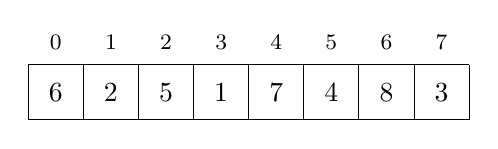
\begin{tikzpicture}[scale=0.7]
\draw (0,0) grid (8,1);
\node at (0.5,0.5) {$6$};
\node at (1.5,0.5) {$2$};
\node at (2.5,0.5) {$5$};
\node at (3.5,0.5) {$1$};
\node at (4.5,0.5) {$7$};
\node at (5.5,0.5) {$4$};
\node at (6.5,0.5) {$8$};
\node at (7.5,0.5) {$3$};

\footnotesize
\node at (0.5,1.4) {$0$};
\node at (1.5,1.4) {$1$};
\node at (2.5,1.4) {$2$};
\node at (3.5,1.4) {$3$};
\node at (4.5,1.4) {$4$};
\node at (5.5,1.4) {$5$};
\node at (6.5,1.4) {$6$};
\node at (7.5,1.4) {$7$};
\end{tikzpicture}
\end{center}
the longest increasing subsequence
contains 4 elements:
\begin{center}
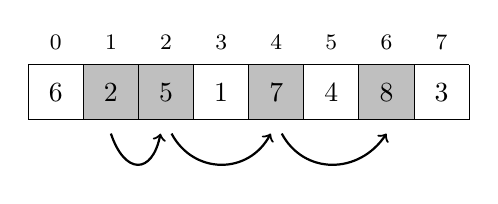
\begin{tikzpicture}[scale=0.7]
\fill[color=lightgray] (1,0) rectangle (2,1);
\fill[color=lightgray] (2,0) rectangle (3,1);
\fill[color=lightgray] (4,0) rectangle (5,1);
\fill[color=lightgray] (6,0) rectangle (7,1);
\draw (0,0) grid (8,1);
\node at (0.5,0.5) {$6$};
\node at (1.5,0.5) {$2$};
\node at (2.5,0.5) {$5$};
\node at (3.5,0.5) {$1$};
\node at (4.5,0.5) {$7$};
\node at (5.5,0.5) {$4$};
\node at (6.5,0.5) {$8$};
\node at (7.5,0.5) {$3$};

\draw[thick,->] (1.5,-0.25) .. controls (1.75,-1.00) and (2.25,-1.00) .. (2.4,-0.25);
\draw[thick,->] (2.6,-0.25) .. controls (3.0,-1.00) and (4.0,-1.00) .. (4.4,-0.25);
\draw[thick,->] (4.6,-0.25) .. controls (5.0,-1.00) and (6.0,-1.00) .. (6.5,-0.25);

\footnotesize
\node at (0.5,1.4) {$0$};
\node at (1.5,1.4) {$1$};
\node at (2.5,1.4) {$2$};
\node at (3.5,1.4) {$3$};
\node at (4.5,1.4) {$4$};
\node at (5.5,1.4) {$5$};
\node at (6.5,1.4) {$6$};
\node at (7.5,1.4) {$7$};
\end{tikzpicture}
\end{center}

Let $\texttt{length}(k)$ denote
the length of the
longest increasing subsequence
that ends at position $k$.
Thus, if we calculate all values of
$\texttt{length}(k)$ where $0 \le k \le n-1$,
we will find out the length of the
longest increasing subsequence.
For example, the values of the function
for the above array are as follows:
\[
\begin{array}{lcl}
\texttt{length}(0) & = & 1 \\
\texttt{length}(1) & = & 1 \\
\texttt{length}(2) & = & 2 \\
\texttt{length}(3) & = & 1 \\
\texttt{length}(4) & = & 3 \\
\texttt{length}(5) & = & 2 \\
\texttt{length}(6) & = & 4 \\
\texttt{length}(7) & = & 2 \\
\end{array}
\]

For example, $\texttt{length}(6)=4$,
because the longest increasing subsequence
that ends at position 6 consists of 4 elements.

To calculate a value of $\texttt{length}(k)$,
we should find a position $i<k$
for which $\texttt{array}[i]<\texttt{array}[k]$
and $\texttt{length}(i)$ is as large as possible.
Then we know that
$\texttt{length}(k)=\texttt{length}(i)+1$,
because this is an optimal way to add
$\texttt{array}[k]$ to a subsequence.
However, if there is no such position $i$,
then $\texttt{length}(k)=1$,
which means that the subsequence only contains
$\texttt{array}[k]$.

Since all values of the function can be calculated
from its smaller values,
we can use dynamic programming.
In the following code, the values
of the function will be stored in an array
$\texttt{length}$.

\begin{lstlisting}
for (int k = 0; k < n; k++) {
    length[k] = 1;
    for (int i = 0; i < k; i++) {
        if (array[i] < array[k]) {
            length[k] = max(length[k],length[i]+1);
        }
    }
}
\end{lstlisting}

This code works in $O(n^2)$ time,
because it consists of two nested loops.
However, it is also possible to implement
the dynamic programming calculation
more efficiently in $O(n \log n)$ time.
Can you find a way to do this?

\section{Paths in a grid}

Our next problem is to find a path
from the upper-left corner to
the lower-right corner
of an $n \times n$ grid, such that
we only move down and right.
Each square contains a positive integer,
and the path should be constructed so
that the sum of the values along
the path is as large as possible.

The following picture shows an optimal
path in a grid:
\begin{center}
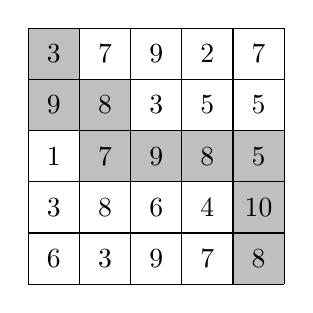
\begin{tikzpicture}[scale=.65]
  \begin{scope}
    \fill [color=lightgray] (0, 9) rectangle (1, 8);
    \fill [color=lightgray] (0, 8) rectangle (1, 7);
    \fill [color=lightgray] (1, 8) rectangle (2, 7);
    \fill [color=lightgray] (1, 7) rectangle (2, 6);
    \fill [color=lightgray] (2, 7) rectangle (3, 6);
    \fill [color=lightgray] (3, 7) rectangle (4, 6);
    \fill [color=lightgray] (4, 7) rectangle (5, 6);
    \fill [color=lightgray] (4, 6) rectangle (5, 5);
    \fill [color=lightgray] (4, 5) rectangle (5, 4);
    \draw (0, 4) grid (5, 9);
    \node at (0.5,8.5) {3};
    \node at (1.5,8.5) {7};
    \node at (2.5,8.5) {9};
    \node at (3.5,8.5) {2};
    \node at (4.5,8.5) {7};
    \node at (0.5,7.5) {9};
    \node at (1.5,7.5) {8};
    \node at (2.5,7.5) {3};
    \node at (3.5,7.5) {5};
    \node at (4.5,7.5) {5};
    \node at (0.5,6.5) {1};
    \node at (1.5,6.5) {7};
    \node at (2.5,6.5) {9};
    \node at (3.5,6.5) {8};
    \node at (4.5,6.5) {5};
    \node at (0.5,5.5) {3};
    \node at (1.5,5.5) {8};
    \node at (2.5,5.5) {6};
    \node at (3.5,5.5) {4};
    \node at (4.5,5.5) {10};
    \node at (0.5,4.5) {6};
    \node at (1.5,4.5) {3};
    \node at (2.5,4.5) {9};
    \node at (3.5,4.5) {7};
    \node at (4.5,4.5) {8};
  \end{scope}
\end{tikzpicture}
\end{center}
The sum of the values on the path is 67,
and this is the largest possible sum on a path
from the
upper-left corner to the lower-right corner.

Assume that the rows and columns of the
grid are numbered from 1 to $n$,
and $\texttt{value}[y][x]$ equals the value
of square $(y,x)$.
Let $\texttt{sum}(y,x)$ denote the maximum
sum on a path from the upper-left corner
to square $(y,x)$.
Now $\texttt{sum}(n,n)$ tells us
the maximum sum
from the upper-left corner to
the lower-right corner.
For example, in the above grid,
$\texttt{sum}(5,5)=67$.

We can recursively calculate the sums
as follows:
\[ \texttt{sum}(y,x) = \max(\texttt{sum}(y,x-1),\texttt{sum}(y-1,x))+\texttt{value}[y][x]\]


The recursive formula is based on the observation
that a path that ends at square $(y,x)$
can come either from square $(y,x-1)$
or square $(y-1,x)$:
\begin{center}
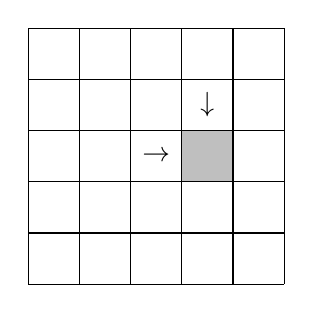
\begin{tikzpicture}[scale=.65]
  \begin{scope}
    \fill [color=lightgray] (3, 7) rectangle (4, 6);
    \draw (0, 4) grid (5, 9);
    
    \node at (2.5,6.5) {$\rightarrow$};
    \node at (3.5,7.5) {$\downarrow$};
    
  \end{scope}
\end{tikzpicture}
\end{center}

Thus, we select the direction that maximizes
the sum.
We assume that $\texttt{sum}(y,x)=0$
if $y=0$ or $x=0$ (because no such paths exist),
so the recursive formula also works when $y=1$ or $x=1$.

Since the function \texttt{sum} has two parameters,
the dynamic programming array also has two dimensions.
For example, we can use an array
\begin{lstlisting}
int sum[N][N];
\end{lstlisting}
and calculate the sums as follows:
\begin{lstlisting}
for (int y = 1; y <= n; y++) {
    for (int x = 1; x <= n; x++) {
        sum[y][x] = max(sum[y][x-1],sum[y-1][x])+value[y][x];
    }
}
\end{lstlisting}
The time complexity of the algorithm is $O(n^2)$.

\section{Knapsack problems}

\index{knapsack}

The term \key{knapsack} refers to problems where
a set of objects is given, and 
subsets with some properties
have to be found.
Knapsack problems can often be solved
using dynamic programming.

In this section, we focus on the following
problem: Given a list of weights
$[w_1,w_2,\ldots,w_n]$,
determine all
sums that can be constructed using the weights.
For example, if the weights are
$[1,3,3,5]$, the following sums are possible:

\begin{center}
\begin{tabular}{rrrrrrrrrrrrr}
 0 & 1 & 2 & 3 & 4 & 5 & 6 & 7 & 8 & 9 & 10 & 11 & 12 \\
\hline
 X & X & & X & X & X & X & X & X & X & & X & X \\
\end{tabular}
\end{center}

In this case, all sums between $0 \ldots 12$
are possible, except 2 and 10.
For example, the sum 7 is possible because we
can select the weights $[1,3,3]$.

To solve the problem, we focus on subproblems
where we only use the first $k$ weights
to construct sums.
Let $\texttt{possible}(x,k)=\textrm{true}$ if
we can construct a sum $x$
using the first $k$ weights,
and otherwise $\texttt{possible}(x,k)=\textrm{false}$.
The values of the function can be recursively
calculated as follows:
\[ \texttt{possible}(x,k) = \texttt{possible}(x-w_k,k-1) \lor \texttt{possible}(x,k-1) \]
The formula is based on the fact that we can
either use or not use the weight $w_k$ in the sum.
If we use $w_k$, the remaining task is to
form the sum $x-w_k$ using the first $k-1$ weights,
and if we do not use $w_k$,
the remaining task is to form the sum $x$
using the first $k-1$ weights.
As the base cases,
\begin{equation*}
    \texttt{possible}(x,0) = \begin{cases}
               \textrm{true}    & x = 0\\
               \textrm{false}   & x \neq 0 \\
           \end{cases}
\end{equation*}
because if no weights are used,
we can only form the sum 0.

The following table shows all values of the function
for the weights $[1,3,3,5]$ (the symbol ''X''
indicates the true values):

\begin{center}
\begin{tabular}{r|rrrrrrrrrrrrr}
$k \backslash x$ & 0 & 1 & 2 & 3 & 4 & 5 & 6 & 7 & 8 & 9 & 10 & 11 & 12 \\
\hline
 0 & X & \\
 1 & X & X \\
 2 & X & X & & X & X \\
 3 & X & X & & X & X & & X & X \\
 4 & X & X & & X & X & X & X & X & X & X & & X & X \\
\end{tabular}
\end{center}

After calculating those values, $\texttt{possible}(x,n)$
tells us whether we can construct a
sum $x$ using \emph{all} weights.

Let $W$ denote the total sum of the weights.
The following $O(nW)$ time
dynamic programming solution
corresponds to the recursive function:
\begin{lstlisting}
possible[0][0] = true;
for (int k = 1; k <= n; k++) {
    for (int x = 0; x <= W; x++) {
        if (x-w[k] >= 0) possible[x][k] |= possible[x-w[k]][k-1];
        possible[x][k] |= possible[x][k-1];
    }
}
\end{lstlisting}

However, here is a better implementation that only uses
a one-dimensional array $\texttt{possible}[x]$
that indicates whether we can construct a subset with sum $x$.
The trick is to update the array from right to left for
each new weight:
\begin{lstlisting}
possible[0] = true;
for (int k = 1; k <= n; k++) {
    for (int x = W; x >= 0; x--) {
        if (possible[x]) possible[x+w[k]] = true;
    }
}
\end{lstlisting}

Note that the general idea presented here can be used
in many knapsack problems.
For example, if we are given objects with weights and values,
we can determine for each weight sum the maximum value
sum of a subset.

\section{Edit distance}

\index{edit distance}
\index{Levenshtein distance}

The \key{edit distance} or \key{Levenshtein distance}\footnote{The distance
is named after V. I. Levenshtein who studied it in connection with binary codes \cite{lev66}.}
is the minimum number of editing operations
needed to transform a string
into another string.
The allowed editing operations are as follows:
\begin{itemize}
\item insert a character (e.g. \texttt{ABC} $\rightarrow$ \texttt{ABCA})
\item remove a character (e.g. \texttt{ABC} $\rightarrow$ \texttt{AC})
\item modify a character (e.g. \texttt{ABC} $\rightarrow$ \texttt{ADC})
\end{itemize}

For example, the edit distance between
\texttt{LOVE} and \texttt{MOVIE} is 2,
because we can first perform the operation
 \texttt{LOVE} $\rightarrow$ \texttt{MOVE}
(modify) and then the operation
\texttt{MOVE} $\rightarrow$ \texttt{MOVIE}
(insert).
This is the smallest possible number of operations,
because it is clear that only one operation is not enough.

Suppose that we are given a string \texttt{x}
of length $n$ and a string \texttt{y} of length $m$,
and we want to calculate the edit distance between
\texttt{x} and \texttt{y}.
To solve the problem, we define a function
$\texttt{distance}(a,b)$ that gives the
edit distance between prefixes
$\texttt{x}[0 \ldots a]$ and $\texttt{y}[0 \ldots b]$.
Thus, using this function, the edit distance
between \texttt{x} and \texttt{y} equals $\texttt{distance}(n-1,m-1)$.

We can calculate values of \texttt{distance}
as follows:
\begin{equation*}
\begin{split}
\texttt{distance}(a,b) = \min(& \texttt{distance}(a,b-1)+1, \\
                           & \texttt{distance}(a-1,b)+1, \\
                           & \texttt{distance}(a-1,b-1)+\texttt{cost}(a,b)).
\end{split}
\end{equation*}
Here $\texttt{cost}(a,b)=0$ if $\texttt{x}[a]=\texttt{y}[b]$,
and otherwise $\texttt{cost}(a,b)=1$.
The formula considers the following ways to
edit the string \texttt{x}:
\begin{itemize}
\item $\texttt{distance}(a,b-1)$: insert a character at the end of \texttt{x}
\item $\texttt{distance}(a-1,b)$: remove the last character from \texttt{x}
\item $\texttt{distance}(a-1,b-1)$: match or modify the last character of \texttt{x}
\end{itemize}
In the two first cases, one editing operation is needed
(insert or remove).
In the last case, if $\texttt{x}[a]=\texttt{y}[b]$,
we can match the last characters without editing,
and otherwise one editing operation is needed (modify).

The following table shows the values of \texttt{distance}
in the example case:
\begin{center}
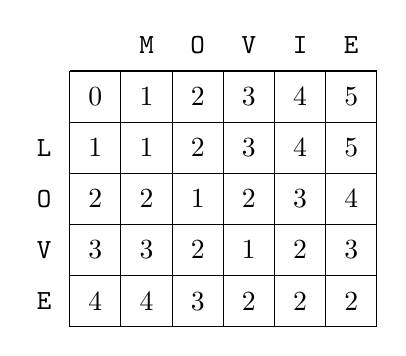
\begin{tikzpicture}[scale=.65]
  \begin{scope}
    %\fill [color=lightgray] (5, -3) rectangle (6, -4);
    \draw (1, -1) grid (7, -6);
    
    \node at (0.5,-2.5) {\texttt{L}};
    \node at (0.5,-3.5) {\texttt{O}};
    \node at (0.5,-4.5) {\texttt{V}};
    \node at (0.5,-5.5) {\texttt{E}};

    \node at (2.5,-0.5) {\texttt{M}};
    \node at (3.5,-0.5) {\texttt{O}};
    \node at (4.5,-0.5) {\texttt{V}};
    \node at (5.5,-0.5) {\texttt{I}};
    \node at (6.5,-0.5) {\texttt{E}};

    \node at (1.5,-1.5) {$0$};
    \node at (1.5,-2.5) {$1$};
    \node at (1.5,-3.5) {$2$};
    \node at (1.5,-4.5) {$3$};
    \node at (1.5,-5.5) {$4$};
    \node at (2.5,-1.5) {$1$};
    \node at (2.5,-2.5) {$1$};
    \node at (2.5,-3.5) {$2$};
    \node at (2.5,-4.5) {$3$};
    \node at (2.5,-5.5) {$4$};
    \node at (3.5,-1.5) {$2$};
    \node at (3.5,-2.5) {$2$};
    \node at (3.5,-3.5) {$1$};
    \node at (3.5,-4.5) {$2$};
    \node at (3.5,-5.5) {$3$};
    \node at (4.5,-1.5) {$3$};
    \node at (4.5,-2.5) {$3$};
    \node at (4.5,-3.5) {$2$};
    \node at (4.5,-4.5) {$1$};
    \node at (4.5,-5.5) {$2$};
    \node at (5.5,-1.5) {$4$};
    \node at (5.5,-2.5) {$4$};
    \node at (5.5,-3.5) {$3$};
    \node at (5.5,-4.5) {$2$};
    \node at (5.5,-5.5) {$2$};
    \node at (6.5,-1.5) {$5$};
    \node at (6.5,-2.5) {$5$};
    \node at (6.5,-3.5) {$4$};
    \node at (6.5,-4.5) {$3$};
    \node at (6.5,-5.5) {$2$};
  \end{scope}
\end{tikzpicture}
\end{center}

The lower-right corner of the table
tells us that the edit distance between
\texttt{LOVE} and \texttt{MOVIE} is 2.
The table also shows how to construct
the shortest sequence of editing operations.
In this case the path is as follows:

\begin{center}
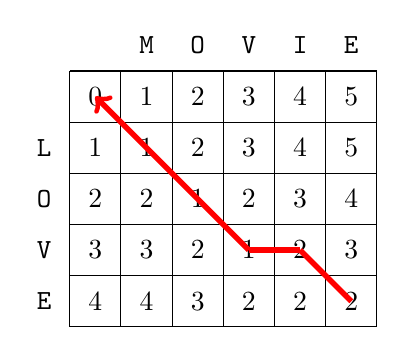
\begin{tikzpicture}[scale=.65]
  \begin{scope}
    \draw (1, -1) grid (7, -6);
    
    \node at (0.5,-2.5) {\texttt{L}};
    \node at (0.5,-3.5) {\texttt{O}};
    \node at (0.5,-4.5) {\texttt{V}};
    \node at (0.5,-5.5) {\texttt{E}};

    \node at (2.5,-0.5) {\texttt{M}};
    \node at (3.5,-0.5) {\texttt{O}};
    \node at (4.5,-0.5) {\texttt{V}};
    \node at (5.5,-0.5) {\texttt{I}};
    \node at (6.5,-0.5) {\texttt{E}};

    \node at (1.5,-1.5) {$0$};
    \node at (1.5,-2.5) {$1$};
    \node at (1.5,-3.5) {$2$};
    \node at (1.5,-4.5) {$3$};
    \node at (1.5,-5.5) {$4$};
    \node at (2.5,-1.5) {$1$};
    \node at (2.5,-2.5) {$1$};
    \node at (2.5,-3.5) {$2$};
    \node at (2.5,-4.5) {$3$};
    \node at (2.5,-5.5) {$4$};
    \node at (3.5,-1.5) {$2$};
    \node at (3.5,-2.5) {$2$};
    \node at (3.5,-3.5) {$1$};
    \node at (3.5,-4.5) {$2$};
    \node at (3.5,-5.5) {$3$};
    \node at (4.5,-1.5) {$3$};
    \node at (4.5,-2.5) {$3$};
    \node at (4.5,-3.5) {$2$};
    \node at (4.5,-4.5) {$1$};
    \node at (4.5,-5.5) {$2$};
    \node at (5.5,-1.5) {$4$};
    \node at (5.5,-2.5) {$4$};
    \node at (5.5,-3.5) {$3$};
    \node at (5.5,-4.5) {$2$};
    \node at (5.5,-5.5) {$2$};
    \node at (6.5,-1.5) {$5$};
    \node at (6.5,-2.5) {$5$};
    \node at (6.5,-3.5) {$4$};
    \node at (6.5,-4.5) {$3$};
    \node at (6.5,-5.5) {$2$};

    \path[draw=red,thick,-,line width=2pt] (6.5,-5.5) -- (5.5,-4.5);
    \path[draw=red,thick,-,line width=2pt] (5.5,-4.5) -- (4.5,-4.5);
    \path[draw=red,thick,->,line width=2pt] (4.5,-4.5) -- (1.5,-1.5);
  \end{scope}
\end{tikzpicture}
\end{center}

The last characters of \texttt{LOVE} and \texttt{MOVIE}
are equal, so the edit distance between them
equals the edit distance between \texttt{LOV} and \texttt{MOVI}.
We can use one editing operation to remove the
character \texttt{I} from \texttt{MOVI}.
Thus, the edit distance is one larger than
the edit distance between \texttt{LOV} and \texttt{MOV}, etc.

\section{Counting tilings}

Sometimes the states of a dynamic programming solution
are more complex than fixed combinations of numbers.
As an example,
consider the problem of calculating
the number of distinct ways to
fill an $n \times m$ grid using
$1 \times 2$ and $2 \times 1$ size tiles.
For example, one valid solution
for the $4 \times 7$ grid is
\begin{center}
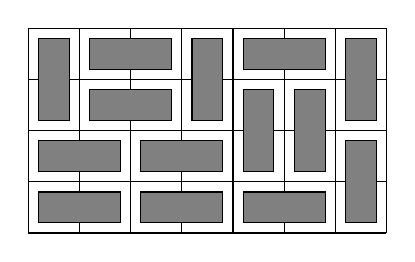
\begin{tikzpicture}[scale=.65]
    \draw (0,0) grid (7,4);
    \draw[fill=gray] (0+0.2,0+0.2) rectangle (2-0.2,1-0.2);
    \draw[fill=gray] (2+0.2,0+0.2) rectangle (4-0.2,1-0.2);
    \draw[fill=gray] (4+0.2,0+0.2) rectangle (6-0.2,1-0.2);
    \draw[fill=gray] (0+0.2,1+0.2) rectangle (2-0.2,2-0.2);
    \draw[fill=gray] (2+0.2,1+0.2) rectangle (4-0.2,2-0.2);
    \draw[fill=gray] (1+0.2,2+0.2) rectangle (3-0.2,3-0.2);
    \draw[fill=gray] (1+0.2,3+0.2) rectangle (3-0.2,4-0.2);
    \draw[fill=gray] (4+0.2,3+0.2) rectangle (6-0.2,4-0.2);

    \draw[fill=gray] (0+0.2,2+0.2) rectangle (1-0.2,4-0.2);
    \draw[fill=gray] (3+0.2,2+0.2) rectangle (4-0.2,4-0.2);
    \draw[fill=gray] (6+0.2,2+0.2) rectangle (7-0.2,4-0.2);
    \draw[fill=gray] (4+0.2,1+0.2) rectangle (5-0.2,3-0.2);
    \draw[fill=gray] (5+0.2,1+0.2) rectangle (6-0.2,3-0.2);
    \draw[fill=gray] (6+0.2,0+0.2) rectangle (7-0.2,2-0.2);

\end{tikzpicture}
\end{center}
and the total number of solutions is 781.

The problem can be solved using dynamic programming
by going through the grid row by row.
Each row in a solution can be represented as a
string that contains $m$ characters from the set
$\{\sqcap, \sqcup, \sqsubset, \sqsupset \}$.
For example, the above solution consists of four rows
that correspond to the following strings:
\begin{itemize}
\item
$\sqcap \sqsubset \sqsupset \sqcap \sqsubset \sqsupset \sqcap$
\item
$\sqcup \sqsubset \sqsupset \sqcup \sqcap \sqcap \sqcup$
\item
$\sqsubset \sqsupset \sqsubset \sqsupset \sqcup \sqcup \sqcap$ 
\item
$\sqsubset \sqsupset \sqsubset \sqsupset \sqsubset \sqsupset \sqcup$
\end{itemize}

Let $\texttt{count}(k,x)$ denote the number of ways to
construct a solution for rows $1 \ldots k$
of the grid such that string $x$ corresponds to row $k$.
It is possible to use dynamic programming here,
because the state of a row is constrained
only by the state of the previous row.

A solution is valid if row $1$ does not contain
the character $\sqcup$,
row $n$ does not contain the character $\sqcap$,
and all consecutive rows are \emph{compatible}.
For example, the rows
$\sqcup \sqsubset \sqsupset \sqcup \sqcap \sqcap \sqcup$ and
$\sqsubset \sqsupset \sqsubset \sqsupset \sqcup \sqcup \sqcap$ 
are compatible, while the rows
$\sqcap \sqsubset \sqsupset \sqcap \sqsubset \sqsupset \sqcap$ and
$\sqsubset \sqsupset \sqsubset \sqsupset \sqsubset \sqsupset \sqcup$
are not compatible.

Since a row consists of $m$ characters and there are
four choices for each character, the number of distinct
rows is at most $4^m$.
Thus, the time complexity of the solution is
$O(n 4^{2m})$ because we can go through the
$O(4^m)$ possible states for each row,
and for each state, there are $O(4^m)$
possible states for the previous row.
In practice, it is a good idea to rotate the grid
so that the shorter side has length $m$,
because the factor $4^{2m}$ dominates the time complexity.

It is possible to make the solution more efficient
by using a more compact representation for the rows.
It turns out that it is sufficient to know which
columns of the previous row contain the upper square
of a vertical tile.
Thus, we can represent a row using only characters
$\sqcap$ and $\Box$, where $\Box$ is a combination
of characters
$\sqcup$, $\sqsubset$ and $\sqsupset$.
Using this representation, there are only
$2^m$ distinct rows and the time complexity is
$O(n 2^{2m})$.

As a final note, there is also a surprising direct formula
for calculating the number of tilings\footnote{Surprisingly,
this formula was discovered in 1961 by two research teams \cite{kas61,tem61}
that worked independently.}:
\[ \prod_{a=1}^{\lceil n/2 \rceil} \prod_{b=1}^{\lceil m/2 \rceil} 4 \cdot (\cos^2 \frac{\pi a}{n + 1} + \cos^2 \frac{\pi b}{m+1})\]
This formula is very efficient, because it calculates
the number of tilings in $O(nm)$ time,
but since the answer is a product of real numbers,
a problem when using the formula is
how to store the intermediate results accurately.


